% CREATED BY DAVID FRISK, 2015
\chapter{Methodology}
\label{methodology}
\lettrine[findent=2pt]{\fbox{\textbf{T}}}{ }his chapter is divided in two phases. Each phase has a data collection, data analysis and the implementation. The  phase II has one more sub-section which involves preparing the questions to interview stakeholders.

%%%%%%
\section{Phase I}

\subsection{Data collection I}
Since Elektra has a lot of data in it, we had to decide on what area to visualize and at which level of abstract. The next sub-section will cover how we ended up deciding on a scope to visualize.

\subsubsection{Identifying a scope to visualize}
As it has been briefly explained in section 2.3, we did the first meeting with Håkan Dahlen at Volvo and he played a big role in identifying the scope of the system to be visualized. We had a long discussion for approximately 2 hours and it was then we figured that we needed to visualize the logical view in Elektra. This view includes the LCs, ports and data elements. \\

If we describe a bit about what is the relationship between ECU and LC is that : first of all, an ECU can have one to many software compositions (SWCs). The SWC is a group of LCs. The LC can have zero to many ports and each port has one data element, it is the data element that connect one LC to another through ports. For example : LC 1 with port 1 can be linked to LC 2 with port 2 only if the port 1 and port 2 has the same data element. Håkan also proposed to visualize the physical view in Elektra which will includes the ECUs.\\

In the discussion with Håkan, we decided to visualize a sub-system. An example of a simple sub-system can be observed from the figure~\ref{fig:hakan-diagram-board} on the top left, there is a small box named SUBSYSTEM and inside of it, there are two ECUs, one ECU has two LCs and another ECU has one LC. The LCs are connected together via ports. The LCs inside the sub-system are also connected to other LCs outside the sub-system but our scope is only for LCs inside a single sub-system. So for this report, we will visualize a sub-system named Visibility Control SPA, this sub-system has 18 LCs and 179 ports at the moment.\\


\begin{figure}[H]
\centering
\captionsetup{justification=centering}
\vspace{0cm}% Adjust vertical spacing here
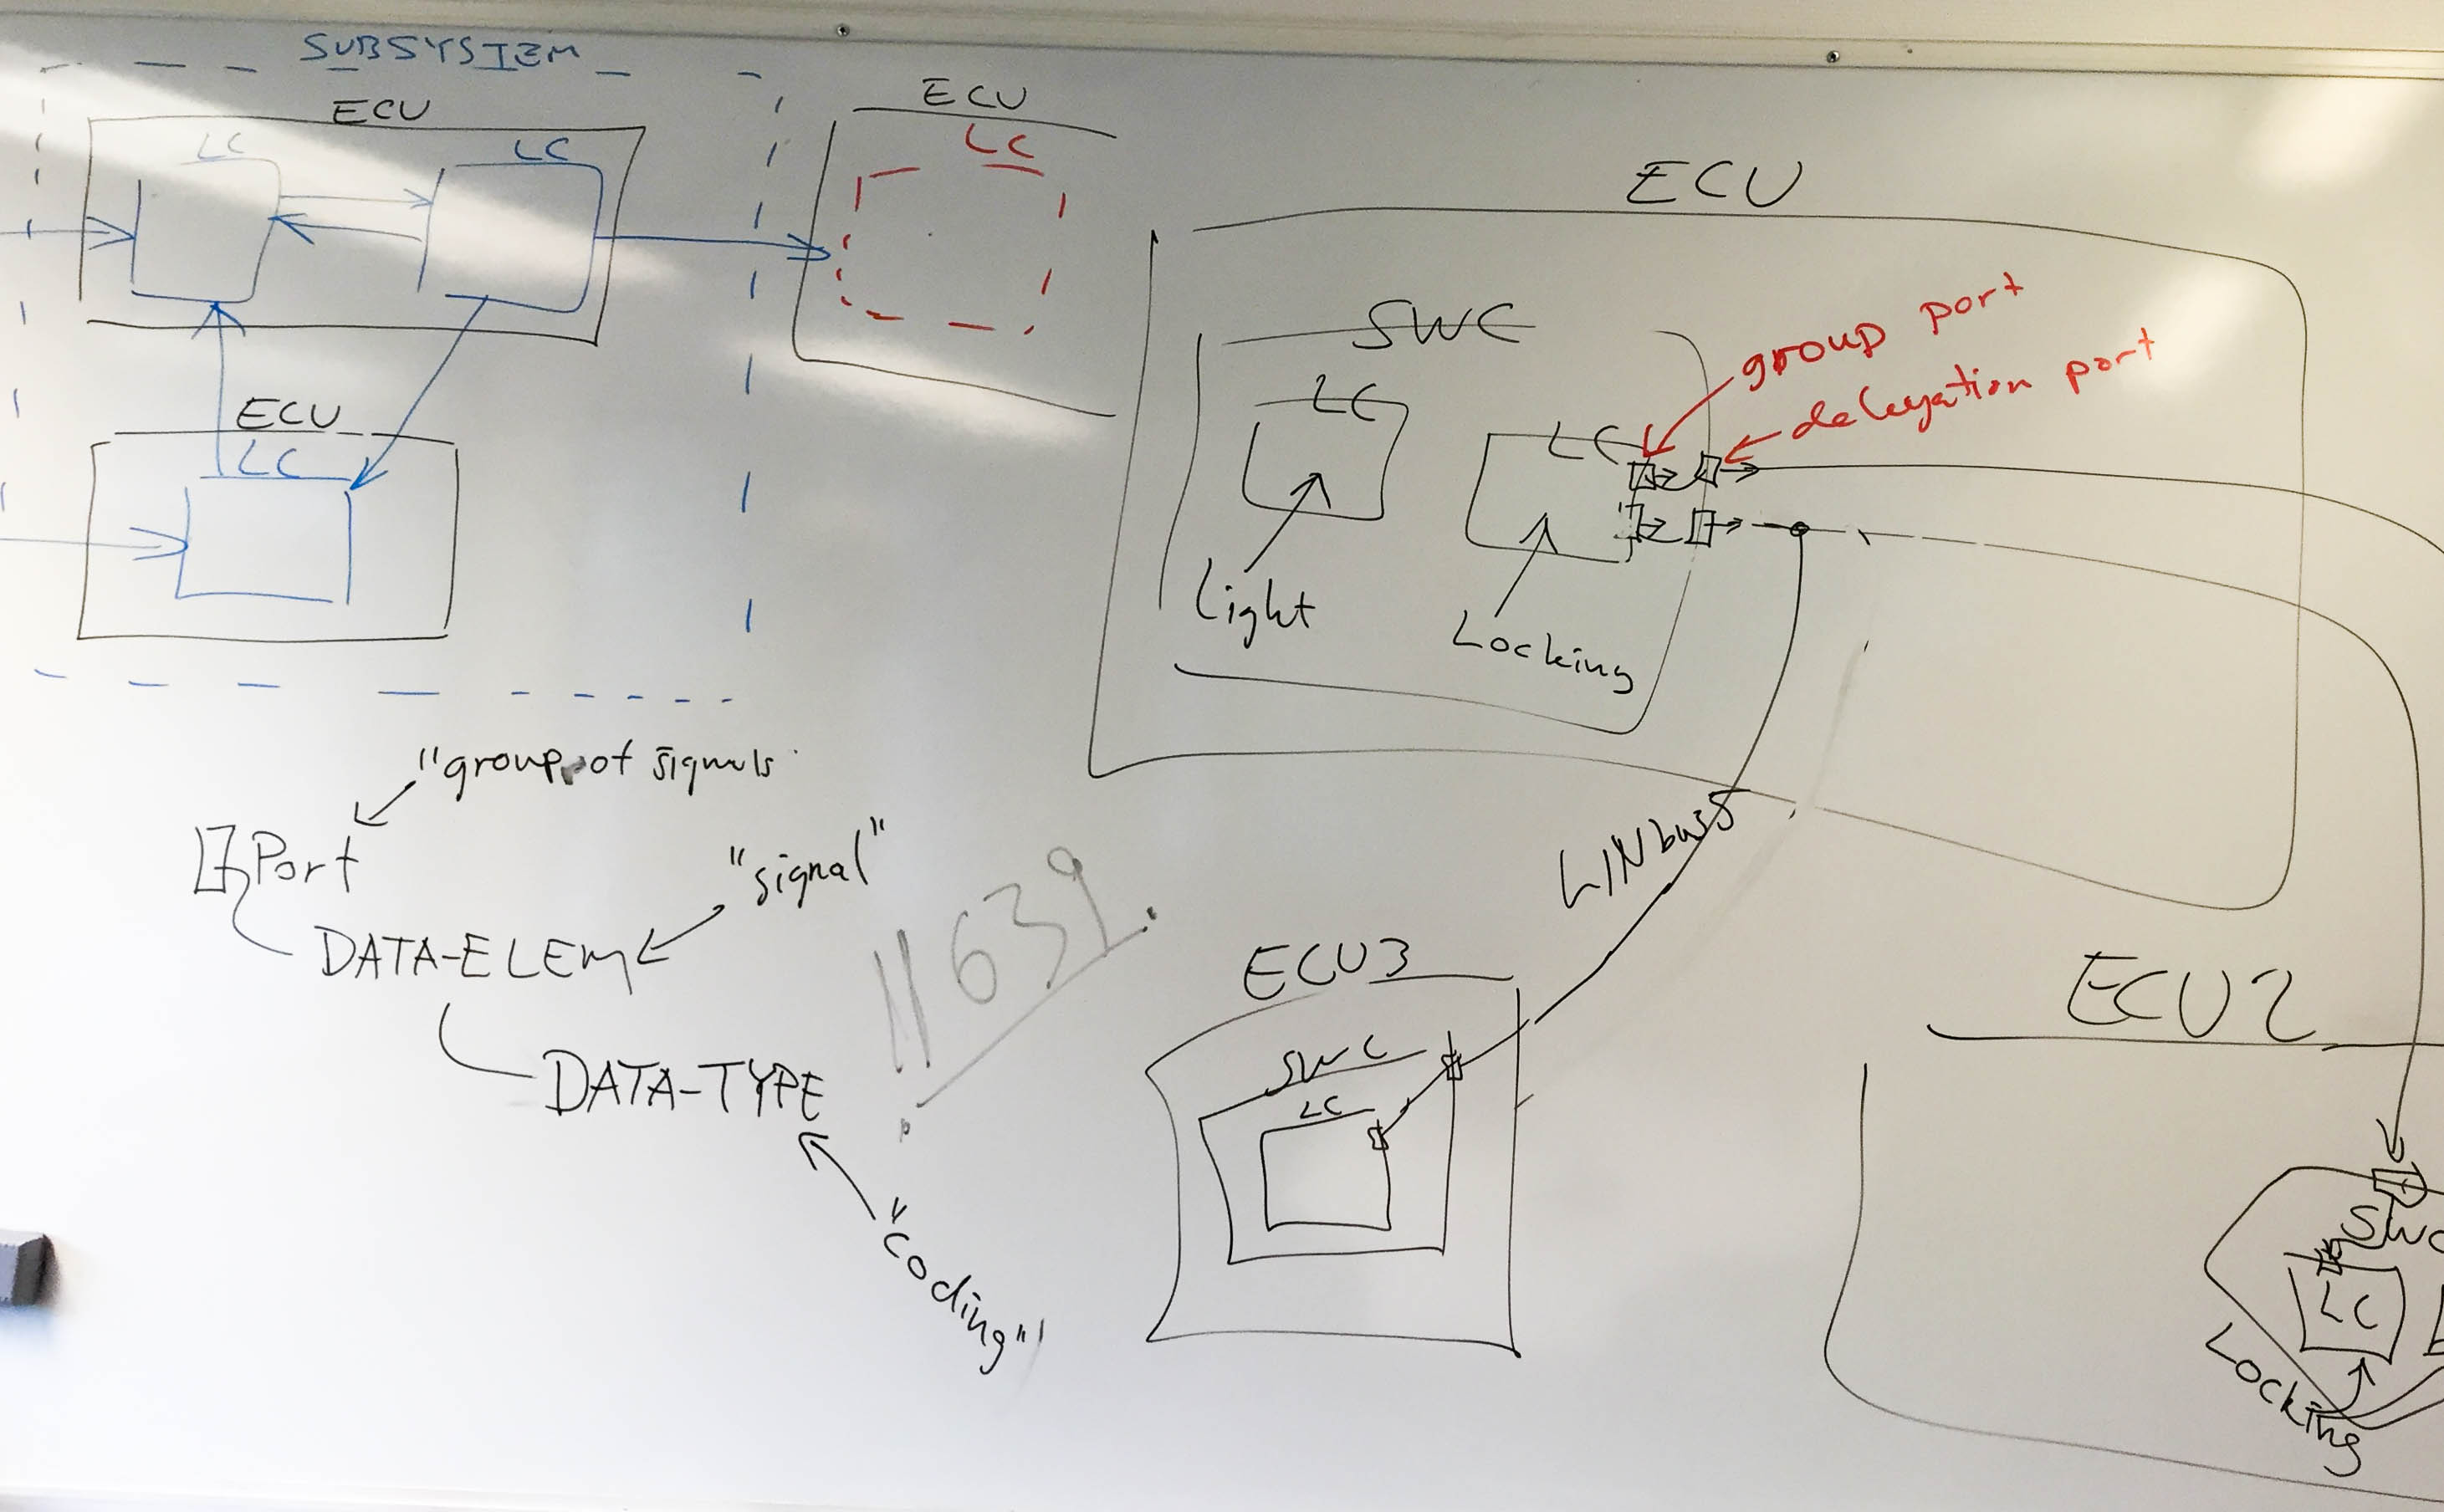
\includegraphics[width=0.85\linewidth]{figure/misc/Hakan.jpg}
\caption{Example of a visualization from a stakeholder}
\label{fig:hakan-diagram-board}
\end{figure}

\subsubsection{Extracting data from Elektra}
The best way that was suggested in retrieving data from Elektra was to use an application program interface(API). At Volvo, we were given a documentation that has a list of APIs and the description of how to use the APIs in order to get the data of your need from Elektra. In order to access the data, one has to be within the Volvo network. Since we did most of our studies outside the company area then we were forced to use the censored data file. The use of API is more dynamic than visualizing a single static file of data. However, this does not make the step to retrieve data from Elektra less meaningful, it is still the same data but later on, a static file will need to be replaced with a specific API url to get the data from Elektra.\\

The data found in the static file retrieved from Elektra is in JavaScript Object Notation(JSON) format. A simple example of JSON object is shown in the  Listing~\ref{code:report_JSON_Object} below :

\begin{lstlisting}[caption=An example of JSON object, label=code:report_JSON_Object]
{
    "id": 1,
    "name": "Master Thesis report",
    "year": 2016,
    "place" : "Sweden",
    "examiner" : "Eric",
    "Supervisors": ["Truong", "Ulf", "Michel","Patrizio"]
}
\end{lstlisting}

%%%%%%
\subsection{Data analysis I}
On this sub-section, we had to understand the meaning of the objects found in the JSON static file and also how most of the objects were connected. The static file had approximately 45 thousands line of code. The beginning of the static file that was retrieved from Elektra is shown in the Listing~\ref{code:origin_static_file} below:

\begin{lstlisting}[caption=A small part of how the original file appear, label=code:origin_static_file]
{
   "elementName": "Visibility Control SPA", 
    "name": "Visibility Control SPA", 
    "state": "In work", 
    "classType": "GSUBSYSTEM", 
    "variant": "MAIN", 
    "domain": "VCC_EEDM", 
    "creationUser": "Anonymous", 
    "className": "SUBSYSTEM", 
    "contentRelations": [
        {
            "destination": {
                "elementName": "LTC 1", 
                "name": "Name for LTC 1", 
                "classType": "GLTC", 
                "variant": "MAIN", 
                "domain": "VCC_EEDM", 
                "creationUser": "Anonymous", 
                "className": "LTC", 
                "state": "Frozen", 
                "modificationUser": "Anonymous", 
                "modificationDate": "2013-06-25T05:13:36+0000", 
                "attributes": {
                    "MaximumLatency": "250", 
                    "Access control": "Access allowed", 
                    "NominalLatency": "-1", 
                    "RefinedConstraints": [], 
                    .....
                }, 
                "creationDate": "2013-05-02T11:48:25+0000", 
                "id": "1937212", 
                "elementId": "1169278", 
                "revision": 0
            }, 
            "contentAttributes": {}
        }, 
        .....   
}
\end{lstlisting}

From the Listing~\ref{code:origin_static_file} shown above, the variable "elementName" that appears on the first row of the JSON file specifies the name of the sub-system that is visualized which has the value "Visibility Control System". You can also notice the variable "className" that appears on the 8th row of the JSON file which has the value "SUBSYSTEM". \\

In order to explain the relationships between JSON objects found in a static flie, we created a meta-model which can help to understand the data found in the file, see figure~\ref{fig:old_metamodel} below.

\begin{figure}[H]
\centering
\captionsetup{justification=centering}
\vspace{0cm}% Adjust vertical spacing here
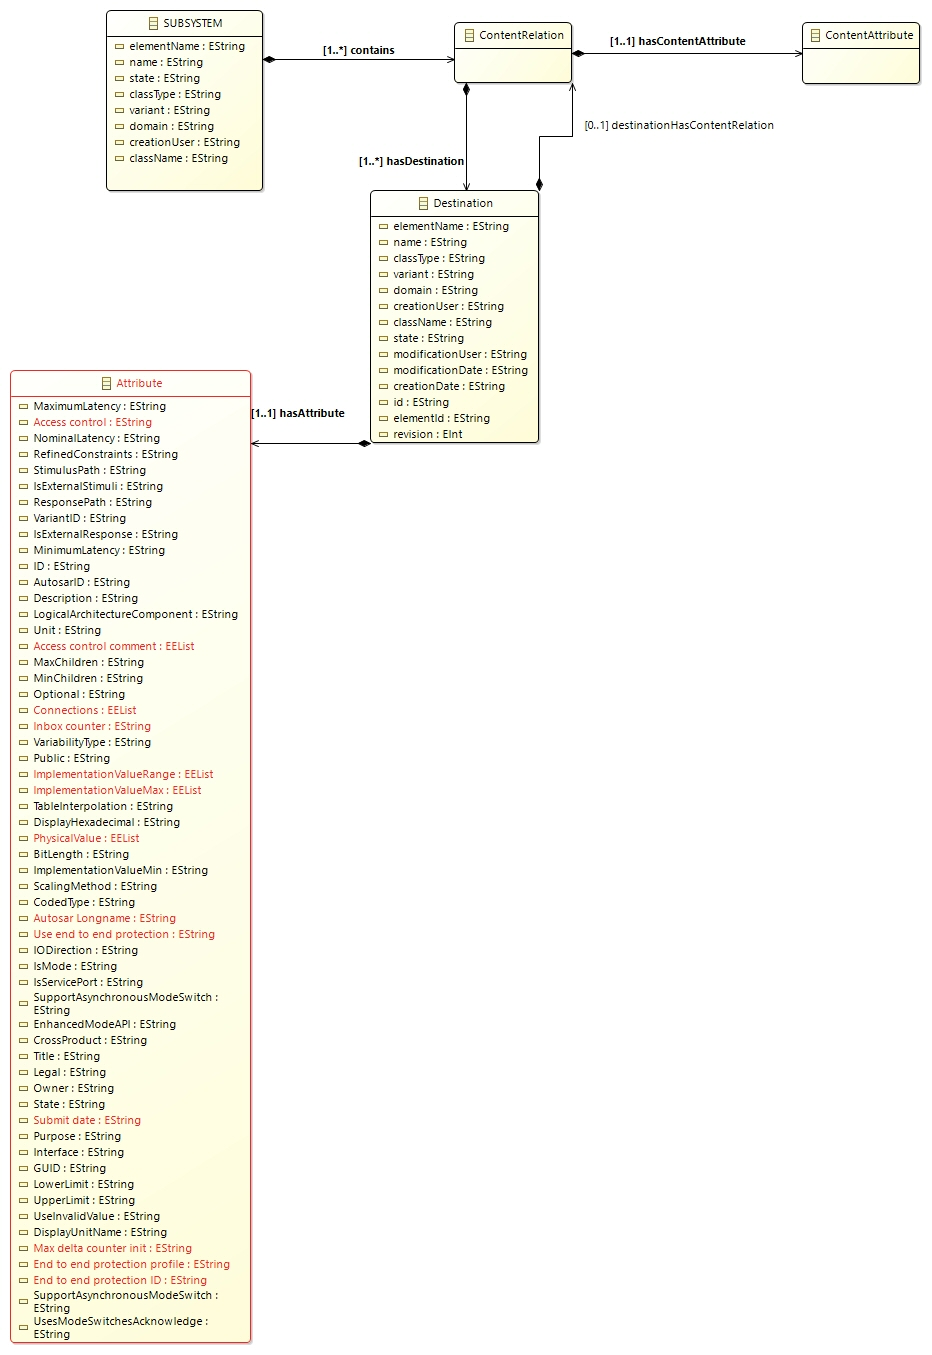
\includegraphics[width=0.85\linewidth]{figure/new_model/Old_Metamodel.jpg}
\caption{Old metamodel}
\label{fig:old_metamodel}
\end{figure}

The meta-model shown in the figure~\ref{fig:old_metamodel} has sum up most of the variables found in the JSON file. The classes that we needed the most are the "contentRelations", "destination" and "attributes". You can notice that the class "contentRelations" has an association of one to many with the class "destination" and also the class "destination" has an association of zero to one with the class "contentRelations". The class "destination" has an association of one to one with the class "attribute". \\

The objects of the class "destination" could be LC, port, data-element, data-type, REQSET, etc. In order to elaborate this, we will give an example of how it appears in a JSON file (see the lists that follows) and the Listing~\ref{code:lc_port_dataElem} after it : \\

\begin{enumerate}
\item a LC which is an object of a class "destination" has an object of a class "contentRelations",call it CR1,
\item an object CR1 can have an array of objects of a class "destinations", a port being one of the object of a class  "destination",
\item a port has an object of a class "contentRelations", call it CR2,
\item an object CR2 can have an array of objects of a class "destinations", a data-element being one of the object of a class "destination",
\item a data-element has an object of a class "contentRelations", call it CR3,
\item an object CR3 can have an array of objects of a class "destinations", a data-type being one of the object of a class "destination", etc \\
\end{enumerate} 


\begin{lstlisting}[caption={A sample part of a JSON file showing the relationship between a LC, a port and a data-element},label=code:lc_port_dataElem]
{
  "destination": {
      "elementName": "LC 1", 
      "name": "Name for LC 1", 
       ....., 
      "contentRelations": [
            {
            "destination": {
                "elementName": "PORT 1", 
                "name": "Name for PORT 1", 
                  ....., 
                 "contentRelations": [
                      {
                      "destination": {
                           "elementName": "DATA-ELEM 1", 
                           "name": "Name for DATA-ELEM 1", 
                            .... 
                           "contentRelations": [
                                 {
                                  "destination": {
                                  "elementName": "DATA-TYPE 1", 
                                  "name": "Name for DATA-TYPE 1",    .....,   
                "attributes": {
                    "IODirection": "REQUIRE",
                    ...
}\\
\end{lstlisting}

If you take a look again at the Listing~\ref{code:lc_port_dataElem}, you can notice a variable with the name "attributes" near the end. This variable has another variable inside of it with the name "IODirection". The variable "IODirection" determines whether a port provides to another port or a port requires another port. The principle in this context of require and provide is that it explains about a dependencies between ports and when it comes to visualize the connection between LCs, we take a look at this variable to determine on how to map the ports in a component diagram. 


\subsubsection{Analyzing the raw JSON data}
The data retrived from Elektra had so many informations that were somehow not needed in the visualization. The first step we did was to find a way to omit the data that was not needed and keep the one that we only needed to visualize and that was the names of the LCs, names of the ports, the value of port that determines whether a port requires another port or a port provides to another port and also we need to keep the data element for each port.

how it looks like, previous meta model, why it doesn't work out \todo{[to be filled in]}


%%%%%%
\subsection{Implementation I}

\subsubsection{Optimizing the raw JSON data}
\todo{[to be filled in]}

\subsubsection{Creating a new meta-model and model instance}
\todo{[to be filled in]}

\subsubsection{Creating a visualization using Acceleo and PlantUML}
\todo{[to be filled in]}


%------------------------------------------------------------------%
%%%%%%
\section{Phase II}

\subsection{Preparing the interview questions}
It was very helpful to identify the goals of study. This had the purpose of understanding well the problem and focus on the things that are useful to our thesis. The article [MTDLG DATA] has explained couple of ways that we followed on resulting to the questions of interests used in the interview. The steps that has been applied for data collection as mentioned in the article were (1) :  Establishing the goals for data collection, (2) : Developing a list of questions of interests and (3) : Establishing data categories.

\subsection{Data collection II}

\subsubsection{Selecting a group of stakeholders}
The visualization tool that the team intended to build has impact on different stakeholders. There are those stakeholders that will be directly affected by the tool and those who will be indirectly affected. We had a single group of stakeholders to interview at the company that contained different categories all grouped together, the categories can be found in the article of community tool box [STK ANALYSIS]. On referring to the article, it describes three different kinds of stakeholders which are primary stakeholders, secondary stakeholders and key stakeholders. Some of the advantages of interviewing the stakeholders include:  getting more ideas, obtaining different perspectives, contribution to us in to avoid misunderstanding of the problem, and also increases the chances of delivering a valuable output to the stakeholders. The primary stakeholders are the people who are directly interacting with Elektra, named beneficiaries and the students (us) who are designing the tool, named the target. The act of visualization can aid the beneficiaries in obtaining a simplified overview of a particular section of Elektra which in turn can provide a quick understanding of the needed components and the interactions between a component and another component. The secondary stakeholders are the ones who are indirectly affected by Elektra. They are the ones who may be affected by the decision made by the stakeholders who interacts directly with Elektra, which in turn will be due to the use of visualization tool on Elektra. Our supervisors at the university can also be in a group of secondary stakeholders, their are not directly interacting with the tool but they also play a greater role in pushing forward our goals for delivering the visualization tool. The key stakeholders are the one funding this project and these can be the two supervisors from the company. All these stakeholders play a very important role in bringing efforts that could result to a better solution of the problem that we intend to resolve.\\
We, who are students and as part of the primary stakeholders (targets), we intended to build a tool that can aid in quick understanding of the architecture and also provide the job opportunity for the need of having such a tool in overview of the architecture. We selected a group of stakeholders to interview. We explained them what were our intentions and what they could provide us to make sure we get the data that we needed.\todo{[to be filled in]}

\subsubsection{Interviewing the selected stakeholders}
\todo{[to be filled in]}

%%%%%%
\subsection{Data analysis II}

\subsubsection{Identifying the needs of the stakeholders}
\todo{[to be filled in]}

\subsubsection{Discovering metrics}
\todo{[to be filled in]}

%%%%%%
\subsection{Implementation II}

\subsubsection{Applying the metrics to the visualization}
\todo{[to be filled in]}
